\documentclass[tikz, border=5mm]{standalone}
\usepackage{tikz}
\usetikzlibrary{calc, arrows.meta, shapes.geometric} % Include necessary libraries

\begin{document}
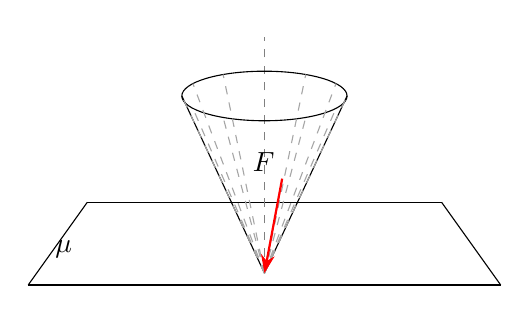
\begin{tikzpicture}[
    scale=1.5, % Adjust overall scale if needed
    >=Stealth, % Use Stealth arrow tips
    force/.style={->, thick, red}, % Style for the force vector F
    axis/.style={-, dashed, gray}, % Style for the normal axis (make it an arrow)
    cone line/.style={-, black}, % Style for cone boundary lines
    cone fill line/.style={-,dashed, gray!70} % Style for lines indicating cone volume
  ]

  % --- Coordinates ---
  \coordinate (contact) at (0,0); % Contact point (origin)

  % --- Surface ---
  % Draw a plane with perspective
  \draw (-2,-0.1) -- (2,-0.1); % Front edge of the surface
  \draw (-1.5,0.6) -- (1.5,0.6); % Back edge of the surface
  \draw (-2,-0.1) -- (-1.5,0.6); % Left edge
  \draw (2,-0.1) -- (1.5,0.6);  % Right edge
  % Label for friction coefficient
  \node at (-1.7, 0.2) {$\mu$};

  % --- Normal Axis (Upwards from the surface) ---
  \coordinate (N_end) at (0, 2); % End point of the normal vector visual representation
  \draw[axis] (contact) -- (N_end) node[right=2pt, black] {}; % Draw normal axis upwards, label N

  % --- Friction Cone (Opening upwards) ---
  \def\coneangle{25} % Define the friction angle (alpha) in degrees (adjust for visual appearance)
  \def\conehight{1.5} % Define the visual height of the cone upwards
  % Calculate cone radius at the base using the angle and height
  \pgfmathsetmacro{\coneradius}{\conehight*tan(\coneangle)}
  % Define the vertical radius of the base ellipse for perspective effect
  \pgfmathsetmacro{\coneellipseY}{0.3*\coneradius}

  % Cone boundary lines (generators)
  \coordinate (C_left) at ({-\coneradius}, \conehight);
  \coordinate (C_right) at ({\coneradius}, \conehight);
  \draw[cone line] (contact) -- (C_left);
  \draw[cone line] (contact) -- (C_right);

  % Cone base ellipse (perspective view) at the top
  \draw[cone line] ($(contact)+(0,\conehight)$) ellipse ({\coneradius} and {\coneellipseY});

  % Internal lines to suggest the cone's volume (originating from contact point)
  % Draw lines to points on the ellipse circumference for better 3D feel
  \foreach \angle in {120, 150, 180, 210, 240} { % Angles on the back part of the ellipse
      \coordinate (p) at ($(contact)+(0,\conehight) + (\angle:{\coneradius} and {\coneellipseY})$);
      \draw[cone fill line] (contact) -- (p);
  }
   \foreach \angle in {-60, -30, 0, 30, 60} { % Angles on the front part of the ellipse
      \coordinate (p) at ($(contact)+(0,\conehight) + (\angle:{\coneradius} and {\coneellipseY})$);
      \draw[cone fill line] (contact) -- (p);
  }
  % Ensure the center axis line is drawn if needed (can use the normal axis)
  % \draw[cone fill line] (contact) -- ($(contact)+(0, \conehight)$); % Center line (optional, covered by N axis)

  % --- Applied Force F (pointing towards contact, within the cone) ---
  % Start point chosen to be inside the cone visually and pointing towards origin
  \coordinate (F_start) at (0.15, 0.8); % Example starting point for F, inside the cone
  \draw[force] (F_start) node[above left=-1pt, black] {$F$} -- (contact); % Draw the force vector F pointing to contact

  % --- Label "Friction cone" ---
  % Position the label above the diagram
%   \node[draw, ellipse] at (0, 2.5) (label) {Friction cone};
  % Arrow pointing from the label to the cone structure
%    \draw [->, shorten >=1pt] (label.south) -- (0, 1.8); % Point towards the top part of the cone/axis

\end{tikzpicture}
\end{document}